% Detaljer hur styrenheten är designad

\section{Styrenhet}

Styrenheten har till uppgift att ta kommandon från huvudenheten och producera utsignaler som motorer och servon kan förstå.

\subsection{Hårdvara}

\begin{figure}[h!]
	\centering
	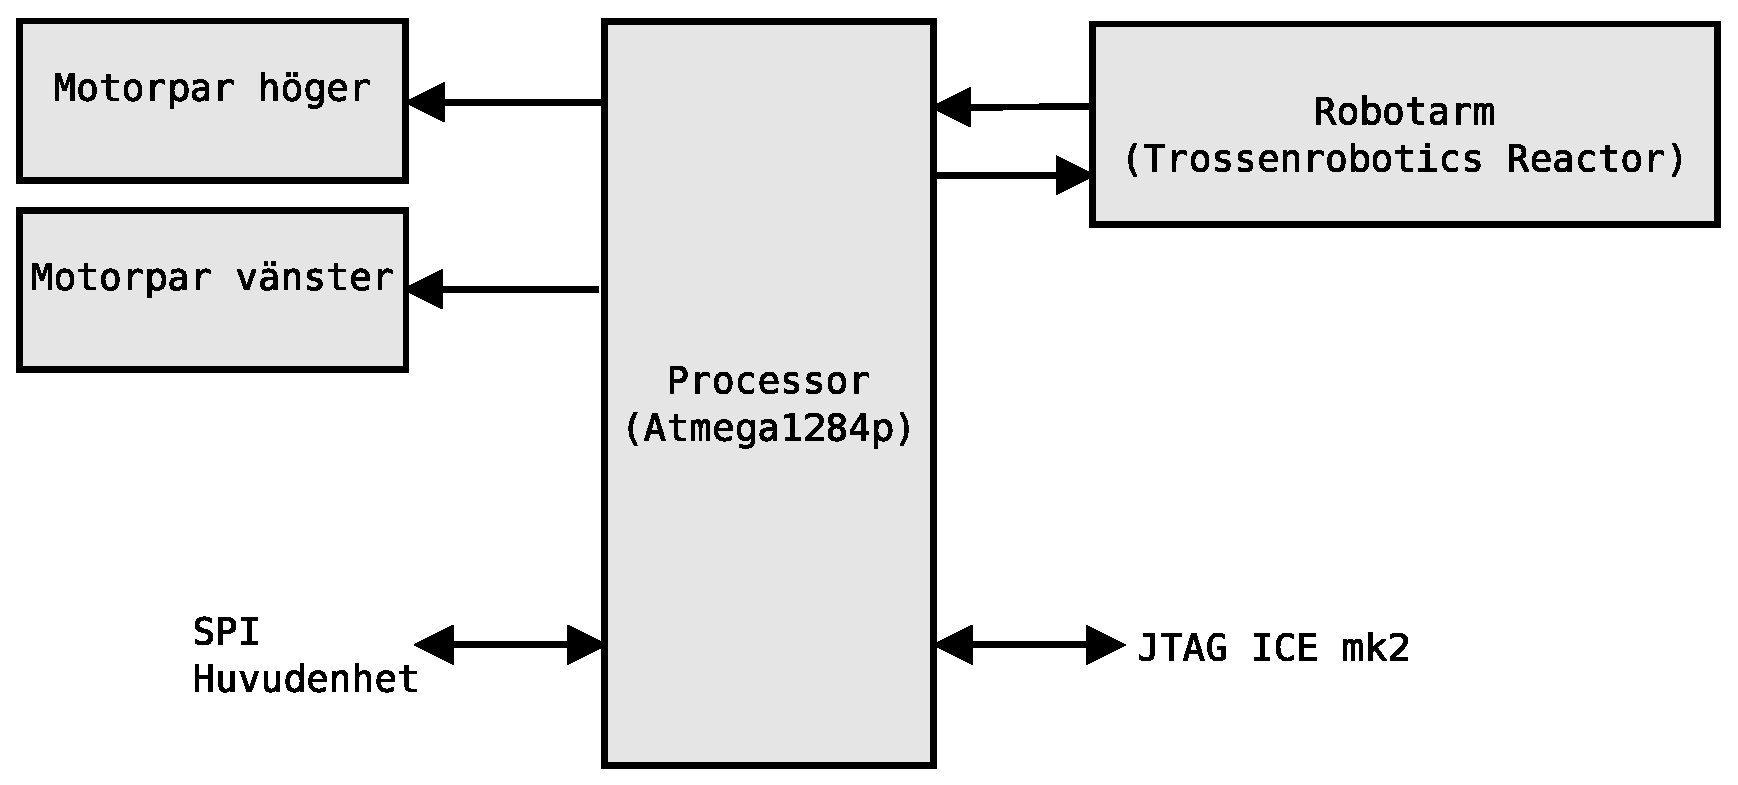
\includegraphics[scale=0.4]{grafik/styrenhet-oversikt}
	\caption{Översikt av styrenheten}
\end{figure}

\begin{figure}[h!]
	\centering
	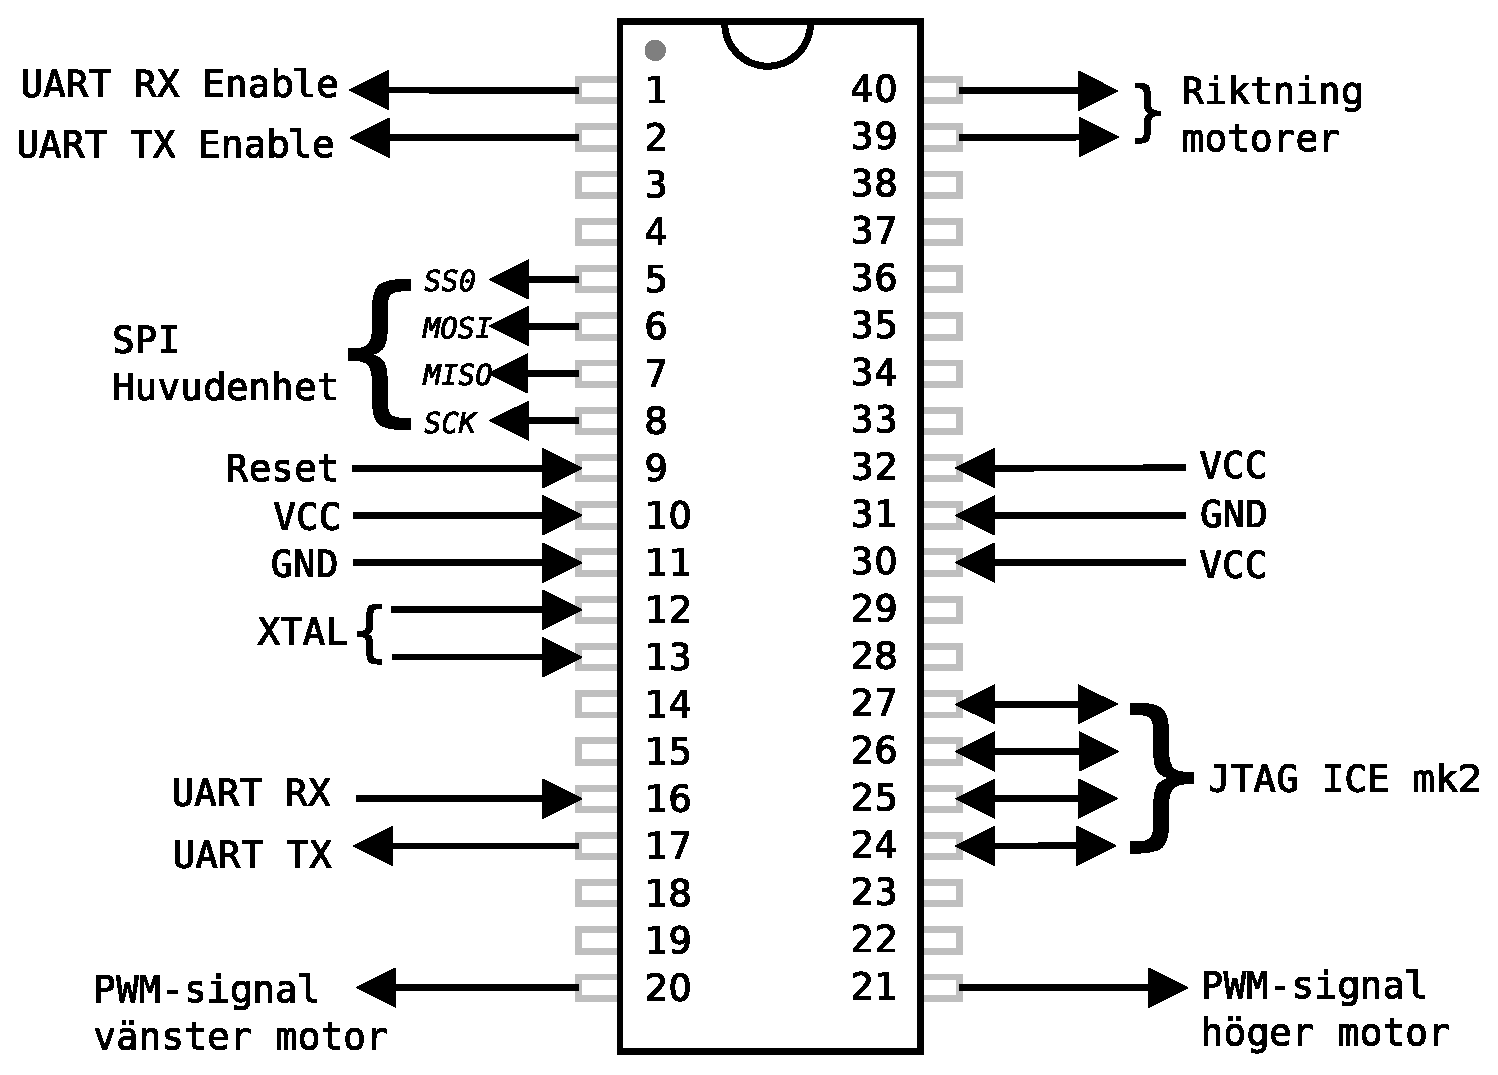
\includegraphics[scale=0.5]{grafik/styrenhet-processor}
	\caption{Schema över hur enkretssdatorn i styrenheten är ansluten till övrig hårdvara.}
\end{figure}

\subsection{Mjukvara}

\todo{Flödesschema styrenheten}
